\documentclass[10pt]{article}
\usepackage{../pplmanual}
%%% Commonly Needed packages
\usepackage{graphicx,color,calc}
\usepackage{fancyvrb}
\usepackage{makeidx}
\usepackage{alltt}
\usepackage[linkbordercolor=(0 0 1),citebordercolor=(0 1 0)]{hyperref}
%%\usepackage{xspace} <- creates problems with other hyperlink packages like "html"

%%% Commands for uniform looks of C++, Charm++, and Projections
\newcommand{\CC}{C\hbox{++}}
\newcommand{\emCC}{C\hbox{\em++}}
\newcommand{\charmpp}{\textsc{Charm++}}
\newcommand{\charmc}{\texttt{charmc}}
\newcommand{\projections}{\textsc{Projections}}
\newcommand{\converse}{\textsc{Converse}}
\newcommand{\ampi}{\textsc{AMPI}}
\newcommand{\tempo}{\textsc{TeMPO}}
\newcommand{\irecv}{\textsl{iRecv}}
\newcommand{\sdag}{\textsl{Structured Dagger}}
\newcommand{\jade}{Jade}

%%% Commands to produce margin symbols
\newcommand{\new}{\marginpar{\fbox{\bf$\mathcal{NEW}$}}}
\newcommand{\important}{\marginpar{\fbox{\bf\Huge !}}}
\newcommand{\experimental}{\marginpar{\fbox{\bf\Huge $\beta$}}}

%%% Commands for manual elements
\newcommand{\zap}[1]{ }
\newcommand{\function}[1]{{\noindent{\textsf{#1}}\\}}
\newcommand{\cmd}[1]{{\noindent{\textsf{#1}}\\}}
\newcommand{\args}[1]{\hspace*{2em}{\texttt{#1}}\\}
\newcommand{\prototype}[1]{\vspace{0.2in}\index{#1}}
\newcommand{\param}[1]{{\texttt{#1}}}
\newcommand{\kw}[1]{{\textsf{#1}\index{#1}}}
\newcommand{\uw}[1]{{\textsl{#1}}}
\newcommand{\desc}[1]{\indent{#1}}
\newcommand{\note}[1]{(\textbf{Note:} #1)}
\newcommand{\term}[1]{{\bf #1}\index{#1}}

\makeindex


\title{BigSim Parallel Simulator for Extremely Large Parallel Machines}
\version{1.01}
	\credits{The Charm++ BigSim Emulator was developed by Arun Singla,
Neelam Saboo and Joshua Unger under the guidance of Prof. L. V. Kale. The new
Converse BigSim Emulator was completely rewritten by Gengbin Zheng. The
Converse BigSim Emulator is the only version under maintenance now. Charm++ and
Adaptive MPI (AMPI) were ported onto the BigSim Emulator by Gengbin Zheng. The
parallel performance simulator was developed by Gengbin Zheng and Gunavardhan
Kakulapati. A postmortem network simulator was developed by Terry Wilmarth,
Eric Bohm and Gengbin Zheng}

\begin{document}
\maketitle

\section{Introduction}

%One approach for building the next generation of parallel computers
%is based on large aggregates of multiprocessor chips with support
%for hardware multithreading. 
%An initial design for IBM's Blue Gene/C project exemplifies this approach.
%Blue Gene/C was a proposed one million processor machine from IBM.

Parallel machines with an extremely large number of processors are now
being designed and built. For example, the BlueGene/L (BG/L) machine
built by IBM has 64,000 dual-processor nodes with 360 teraflops of
peak performance. Another more radical design from IBM,
code-named Cyclops (BlueGene/C), had over one million floating point units,
fed by 8 million instructions streams supported by individual thread units,
targeting 1 petaflops of peak performance.


It is important that one can study the programming issues and performance
of parallel applications on such machines even before the machine is built.
Thus, we have developed a parallel simulator -- BigSim, to facilitate this research.

Since our research was initiated by the BlueGene/C project, in previous
editions of this manual we also called our simulator as Blue Gene Simulator.
Our simulator is capable of simulating a broad class of "Massively Parallel
Processors-In-Memory", or MPPIM machines. 

\subsection{Simulator system components}

Our simulator system includes these components: 
\begin{enumerate}
\item a parallel emulator which emulates a low level machine API targeting an architecture like BlueGene; 
\item a message driven programming language (Charm++) running on top of the emulator; 
\item the Adaptive MPI (an implementation of MPI on top of Charm++) environment; 
\item a parallel post-mortem mode simulator for performance prediction, including network simulation. 
\end{enumerate}

\subsection{History}
	The first version of the BlueGene emulator was written in Charm++, a
parallel object language, in fall 2001.  The second version of the BlueGene
emulator was completely rewritten on top of Converse instead of Charm++ in
spring 2002.  While the API supported by the original emulator remains almost
the same, many new features were added.
% - support of thread-committed messages that 
%can be send to a specific thread in a Blue Gene node; support of Blue Gene
%node level broadcast.
The new emulator was implemented on a portable low layer communication library
- Converse, in order to achieve better performance by avoiding the cross layer
overhead.
%Another advantage is that the lighter weighted emulator makes it easier to
%port higher level of programming language onto the emulator.

	Charm++ was ported to the emulator in 2002, providing the first
parallel language model on top of the emulator.

A performance simulation capability was added to the emulator in spring 2003.
The new simulator was renamed to BigSim at the same time.
During the same year, we developed a POSE-based postmortem mode network
simulator called BigNetSim. In fall 2006, we renamed BigNetSim as simply
BigSim simulator.

In the following sections, we will first describe how to download and compile
the BigSim system (Section~\ref{install}). Section~\ref{bgemulator} describes
the BigSim Emulator and the low level machine API in detail. 


\charmpp{} can be installed either from the source code or using a precompiled
binary package. Building from the source code provides more flexibility, since one 
can choose the options as desired. However, a precompiled binary may be slightly
easier to get running.
 
\section{Downloading \charmpp{}}

\charmpp{} can be downloaded using one of the following methods:

\begin{itemize}
\item From \charmpp{} website -- The current stable version (source code and
binaries) can be downloaded from our website at {\em http://charm.cs.illinois.edu/software}.
\item From source archive -- The latest development version of \charmpp{} can be downloaded
from our source archive using {\em git clone http://charm.cs.illinois.edu/gerrit/charm}.
\end{itemize}

If you download the source code from the website, you will have to unpack it 
using a tool capable of extracting gzip'd tar files, such as tar (on Unix) 
or WinZIP (under Windows).  \charmpp{} will be extracted to a directory 
called ``charm''. 

\section{Installation}

A typical prototype command for building \charmpp{} from the source code is:
\vspace{5pt}\\
{\bf ./build $<$TARGET$>$ $<$TARGET ARCHITECTURE$>$ [OPTIONS]} where,

\begin{description}
\item [TARGET] is the framework one wants to build such as {\em charm++} or {\em
AMPI}.
\item [TARGET ARCHITECTURE] is the machine architecture one wants to build for
such as {\em netlrts-linux-x86\_64}, {\em pamilrts-bluegeneq} etc.
\item [OPTIONS] are additional options to the build process, e.g. {\em smp} is
used to build a shared memory version, {\em -j8} is given to build in parallel
etc.
\end {description}

In Table~\ref{tab:buildlist}, a list of build commands is provided for some of the commonly 
used systems. Note that, in general, options such as {\em smp},
\verb|--with-production|, compiler specifiers etc can be used with all targets.
It is advisable to build with \verb|--with-production| to obtain the best
performance.  If one desires to perform trace collection (for Projections),
\verb|--enable-tracing --enable-tracing-commthread| should also be passed to the
build command.

Details on all the available alternatives for each of the above mentioned
parameters can be found by invoking \verb|./build --help|. One can also go through the
build process in an interactive manner. Run \verb|./build|, and it will be followed by
a few queries to select appropriate choices for the build one wants to perform.


\begin{table}[ht]
\begin{tabular}{|p{6cm}|p{9cm}|}
\hline
Net with 32 bit Linux & \verb|./build charm++ netlrts-linux --with-production -j8|
\\\hline
Multicore (single node, shared memory) 64 bit Linux & \verb|./build charm++ multicore-linux-x86_64 --with-production -j8|
\\\hline
Net with 64 bit Linux & \verb|./build charm++ netlrts-linux-x86_64 --with-production -j8|
\\\hline
Net with 64 bit Linux (intel compilers) & \verb|./build charm++ netlrts-linux-x86_64 icc --with-production -j8|
\\\hline
Net with 64 bit Linux (shared memory) & \verb|./build charm++ netlrts-linux-x86_64 smp --with-production -j8|
\\\hline
Net with 64 bit Linux (checkpoint restart based fault tolerance) & \verb|./build charm++ netlrts-linux-x86_64 syncft --with-production -j8|
\\\hline
MPI with 64 bit Linux & \verb|./build charm++ mpi-linux-x86_64 --with-production -j8|
\\\hline
MPI with 64 bit Linux (shared memory) & \verb|./build charm++ mpi-linux-x86_64 smp --with-production -j8|
\\\hline
MPI with 64 bit Linux (mpicxx wrappers) & \verb|./build charm++ mpi-linux-x86_64 mpicxx --with-production -j8|
\\\hline
IBVERBS with 64 bit Linux & \verb|./build charm++ verbs-linux-x86_64 --with-production -j8|
\\\hline
OFI with 64 bit Linux & \verb|./build charm++ ofi-linux-x86_64 --with-production -j8|
\\\hline
Net with 64 bit Windows & \verb|./build charm++ netlrts-win-x86_64 --with-production -j8|
\\\hline
MPI with 64 bit Windows & \verb|./build charm++ mpi-win-x86_64 --with-production -j8|
\\\hline
Net with 64 bit Mac & \verb|./build charm++ netlrts-darwin-x86_64 --with-production -j8|
\\\hline
Blue Gene/Q (bgclang compilers) & \verb|./build charm++ pami-bluegeneq --with-production -j8|
\\\hline
Blue Gene/Q (bgclang compilers) & \verb|./build charm++ pamilrts-bluegeneq --with-production -j8|
\\\hline
Cray XE6 & \verb|./build charm++ gni-crayxe --with-production -j8|
\\\hline
Cray XK7 & \verb|./build charm++ gni-crayxe-cuda --with-production -j8|
\\\hline
Cray XC40 & \verb|./build charm++ gni-crayxc --with-production -j8|
\\\hline
\end{tabular}
\caption{Build command for some common cases}
\label{tab:buildlist}
\end{table}

As mentioned earlier, one can also build \charmpp{} using the precompiled binary
in a manner similar to what is used for installing any common software.

When a Charm++ build folder has already been generated, it is possible to
perform incremental rebuilds by invoking \verb|make| from the \verb|tmp| folder
inside it. For example, with a {\em netlrts-linux-x86\_64} build, the path
would be \verb|netlrts-linux-x86_64/tmp|. On Linux and macOS, the tmp symlink
in the top-level charm directory also points to the tmp directory of the most
recent build.

Alternatively, CMake can be used for configuring and building Charm++. You can
use \verb|cmake-gui| or \verb|ccmake| for an overview of available options.
Note that some are only effective when passed with \verb|-D| from the
command line while configuring from a blank slate. To build with all defaults,
\verb|cmake .| is sufficient, though invoking CMake from a separate location
(ex: \verb|mkdir mybuild && cd mybuild && cmake ../charm|) is recommended.

The main directories in a \charmpp{} installation are:

\begin{description}
\item[\kw{charm/bin}]
Executables, such as charmc and charmrun,
used by \charmpp{}.

\item[\kw{charm/doc}]
Documentation for \charmpp{}, such as this
document.  Distributed as LaTeX source code; HTML and PDF versions
can be built or downloaded from our web site.

\item[\kw{charm/include}]
The \charmpp{} C++ and Fortran user include files (.h).

\item[\kw{charm/lib}]
The static libraries (.a) that comprise \charmpp{}.

\item[\kw{charm/lib\_so}]
The shared libraries (.so/.dylib) that comprise \charmpp{},
if \charmpp{} is compiled with the \texttt{--build-shared} option.

\item[\kw{charm/examples}]
Example \charmpp{} programs.

\item[\kw{charm/src}]
Source code for \charmpp{} itself.

\item[\kw{charm/tmp}]
Directory where \charmpp{} is built.

\item[\kw{charm/tests}]
Test \charmpp{} programs used by autobuild.

\end{description}

\section{Reducing disk usage}

The charm directory contains a collection of example-programs and
test-programs.  These may be deleted with no other effects. You may
also {\tt strip} all the binaries in {\tt charm/bin}.



\section{Blue Gene Emulator}
\label{bgemulator}

The Blue Gene emulator environment is designed with the following
objectives:

\begin{enumerate}
\item To support a realistic Blue Gene API on existing parallel machines

\item To obtain first-order performance estimates of algorithms

\item To facilitate implementations of alternate programming models for
      Blue Gene
\end{enumerate}

The ``Blue Gene'' machine supported by the emulator consists of
three-dimensional grid of 1-chip nodes.  The user may specify the size
of the machine along each dimension (e.g. 34x34x36).  The chip supports
$k$ threads (e.g. 200), each with its own integer unit.  The proximity of
the integer unit with individual memory modules within a chip is not
currently modeled.

The API supported by the emulator can be broken down into several
components:

\begin{enumerate}
\item Low-level API for chip-to-chip communication
\item Mid-level API that supports local micro-tasking with a chip level
scheduler with features such as: read-only variables, reductions, broadcasts,
distributed tables, get/put operations
\item Migratable objects with automatic load balancing support
\end{enumerate}

Of these, the first two have been implemented.  The simple time stamping
algorithm, without error correction, has been implemented.  More
sophisticated timing algorithms, specifically aimed at error correction,
and more sophisticated features (2, 3, and others), as well as libraries
of commonly needed parallel operations are part of the proposed work for
future.

The following sections define the appropriate parts of the API, with
example programs and instructions for executing them.

\subsection{Blue Gene Programming Environment}

The basic philosophy of the Blue Gene Emulator is to hide intricate details
of the Blue Gene machine from the
application developer. Thus, the application developer needs to provide
intialization details and handler
functions only and gets the result as though running on a real machine.
Communication, Thread creation,
Time Stamping, etc are done by the emulator.

\subsubsection{Blue Gene API: Level 0}

\function{void addBgNodeInbuffer(bgMsg *msgPtr, int nodeID)}
\desc{
        low-level primitive invoked by Blue Gene emulator to put the 
        message to the inbuffer queue of a node.

        msgPtr - pointer to the message to be sent to target node; 

        nodeID - node ID of the target node, it is the serial number of a 
                 bluegene node in the emulator's physical node.
}

\function{void addBgThreadMessage(bgMsg *msgPtr, int threadID)}
\desc{
        add a message to a thread's affinity queue, these messages can be 
 	only executed by a specific thread indicated by threadID.
}

\function{void addBgNodeMessage(bgMsg *msgPtr)}
\desc{
	add a message to a node's non-affinity queue, these messages can be 
	executed by any thread in the node.
}

\function{boolean checkReady()}
\desc{
        invoked by communication thread to see if there is any unattended
        message in inBuffer.
}

\function{bgMsg * getFullBuffer()}
\desc{
	invoked by communication thread to retrieve the unattended message 
	in inBuffer.
}

\function{CmiHandler msgHandlerFunc(char *msg)}
\desc{
	Handler function type that user can register to handle the message.
}

\function{void sendPacket(int x, int y, int z, int msgSize,bgMsg *msg)}
\desc{
	chip-to-chip communication function. It send a message to Node[x][y][z].
        
	bgMsg is the message type with message envelop used internally.
}

\subsubsection{Initialization API: Level 1a}

All the functions defined in API Level 0 are used internally for the 
implementation of bluegene node communication and worker threads.

From this level, the functions defined are exposed to users to write bluegene
programs on the emulator.

Considering that the emulator machine will emulate several Bluegene nodes on
each physical node, the emulator program defines this function 
\function{BgEmulatorInit(int argc, char **argv)} to initialize each emulator
node. In this function, user program can define the Bluegene machine size,
number of communication/worker threads, and check the command line arguments.

The size of the Blue Gene machine being emulated and the number of thread per
node is determined either by the command line arguments or calling following
functions:

\function{void BgSetSize(int sx, int sy, int sz)}
\desc{
	set Blue Gene Machine size;
}

\function{void BgSetNumWorkThread(int num)}
\desc{
	set number of worker threads per node;
}

\function{void BgSetNumCommThread(int num)}
\desc{
	set number of communication threads per node;
}

\function{int BgRegisterHandler(BgHandler h)}
\desc{
	register user message handler functions; 
}

For each Blue Gene node, the execution starts at 
\function{BgNodeStart(int argc, char **argv)} called by the emulator,
where application handlers can be registered and computation 
is triggered by creating a task at required nodes.

Similar to pthread's thread specifc data, each bluegene node has its
own node specific data associated with it. To do this, the user needs to define its 
own node-specific variables encapsulated in a struct definition and register
 the pointer to the data with the emulator by following function:

\function{void BgSetNodeData(char *data)}

To retrieve the node specific data, call:

\function{char *BgGetNodeData();}

After completion of execution, user program invokes a function:

\function{void BgShutdown()}

to terminate the emulator.

\subsubsection{Handler Function API: Level 1a}

The following functions can be called in user's application program to retrieve
the Blue Gene machine information, get thread execution time, and perform
the communication.

\function{void BgGetSize(int *sx, int *sy, int *sz);}

\function{int BgGetNumWorkThread();}

\function{int BgGetNumCommThread();}

\function{int BgGetThreadID();}

\function{double BgGetTime();}

\function{void BgSendPacket(int x, int y, int z, int threadID, int handlerID, WorkType type, int numbytes, char* data);}
\desc{
This sends a trunk of data to Node[x, y, z] and also specifies the
handler function to be used for this message i.e. the handlerID;
threadID specifes the desired thread to handle the message, ANYTHREAD means
no preference.

To specify the thread category:
\begin{description}
\item[1:] a small piece of work that can be done by
communication thread itself, so NO scheduling overhead.
\item[0:] a large piece of work, so communication thread
schedules it for a worker thread
\end{description}
}


\subsection{Writing a Blue Gene Application}

\subsubsection{Application Skeleton}

\begin{alltt}
Handler function prototypes;
Node specific data type declarations;

void  BgEmulatorInit(int argc, char **argv)  function
  Configure bluegene machine parameters including size, number of threads, etc.
  You also neet to register handlers here.

void *BgNodeStart(int argc, char **argv) function
  The usual practice in this function is to send an intial message to trigger 
  the execution.
  You can also register node specific data in this function.

Handler Function 1, void handlerName(char *info)
Hanlder Function 2, void handlerName(char *info)
..
Handler Function N, void handlerName(char *info)

\end{alltt}

\subsubsection{Sample Application 1}

\begin{verbatim}
/* Application: 
 *   Each node starting at [0,0,0] sends a packet to next node in
 *   the ring order.
 *   After node [0,0,0] gets message from last node
 *   in the ring, the application ends.
 */


#include "blue.h"

#define MAXITER 2

int iter = 0;
int passRingHandler;

void passRing(char *msg);

void nextxyz(int x, int y, int z, int *nx, int *ny, int *nz)
{
  int numX, numY, numZ;

  BgGetSize(&numX, &numY, &numZ);
  *nz = z+1; *ny = y; *nx = x;
  if (*nz == numZ) {
    *nz = 0; (*ny) ++;
    if (*ny == numY) {
      *ny = 0; (*nx) ++;
      if (*nx == numX) *nx = 0;
    }
  }
}

void BgEmulatorInit(int argc, char **argv)
{
  passRingHandler = BgRegisterHandler(passRing);
}

/* user defined functions for bgnode start entry */
void BgNodeStart(int argc, char **argv)
{
  int x,y,z;
  int nx, ny, nz;
  int data, id;

  BgGetXYZ(&x, &y, &z);
  nextxyz(x, y, z, &nx, &ny, &nz);
  id = BgGetThreadID();
  data = 888;
  if (x == 0 && y==0 && z==0) {
    BgSendPacket(nx, ny, nz, -1,passRingHandler, LARGE_WORK, 
				sizeof(int), (char *)&data);
  }
}

/* user write code */
void passRing(char *msg)
{
  int x, y, z;
  int nx, ny, nz;
  int id;
  int data = *(int *)msg;

  BgGetXYZ(&x, &y, &z);
  nextxyz(x, y, z, &nx, &ny, &nz);
  if (x==0 && y==0 && z==0) {
    if (++iter == MAXITER) BgShutdown();
  }
  id = BgGetThreadID();
  BgSendPacket(nx, ny, nz, -1, passRingHandler, LARGE_WORK, 
				sizeof(int), (char *)&data);
}

\end{verbatim}


\subsubsection{Sample Application 2}

\begin{verbatim}

/* Application: 
 *   Find the maximum element.
 *   Each node computes maximum of it's elements and
 *   the max values it received from other nodes
 *   and sends the result to next node in the reduction sequence.
 * Reduction Sequence: Reduce max data to X-Y Plane
 *   Reduce max data to Y Axis
 *   Reduce max data to origin.
 */


#include <stdlib.h>
#include "blue.h"

#define A_SIZE 4

#define X_DIM 3
#define Y_DIM 3
#define Z_DIM 3

int REDUCE_HANDLER_ID;
int COMPUTATION_ID;

extern "C" void reduceHandler(char *);
extern "C" void computeMax(char *);

class ReductionMsg {
public:
  int max;
};

class ComputeMsg {
public:
  int dummy;
};

void BgEmulatorInit(int argc, char **argv)
{
  if (argc < 2) { 
    CmiAbort("Usage: <program> <numCommTh> <numWorkTh>\n"); 
  }

  /* set machine configuration */
  BgSetSize(X_DIM, Y_DIM, Z_DIM);
  BgSetNumCommThread(atoi(argv[1]));
  BgSetNumWorkThread(atoi(argv[2]));

  REDUCE_HANDLER_ID = BgRegisterHandler(reduceHandler);
  COMPUTATION_ID = BgRegisterHandler(computeMax);

}

void BgNodeStart(int argc, char **argv) {
  int x, y, z;
  BgGetXYZ(&x, &y, &z);

  ComputeMsg *msg = new ComputeMsg;
  BgSendLocalPacket(ANYTHREAD, COMPUTATION_ID, LARGE_WORK, 
			sizeof(ComputeMsg), (char *)msg);
}

void reduceHandler(char *info) {
  // assumption: THey are initialized to zero?
  static int max[X_DIM][Y_DIM][Z_DIM];
  static int num_msg[X_DIM][Y_DIM][Z_DIM];

  int i,j,k;
  int external_max;

  BgGetXYZ(&i,&j,&k);
  external_max = ((ReductionMsg *)info)->max;
  num_msg[i][j][k]++;

  if ((i == 0) && (j == 0) && (k == 0)) {
    // master node expects 4 messages:
    // 1 from itself;
    // 1 from the i dimension;
    // 1 from the j dimension; and
    // 1 from the k dimension
    if (num_msg[i][j][k] < 4) {
      // not ready yet, so just find the max
      if (max[i][j][k] < external_max) {
	max[i][j][k] = external_max;
      }
    } else {
      // done. Can report max data after making last comparison
      if (max[i][j][k] < external_max) {
	max[i][j][k] = external_max;
      }
      CmiPrintf("The maximal value is %d \n", max[i][j][k]);
      BgShutdown();
      return;
    }
  } else if ((i == 0) && (j == 0) && (k != Z_DIM - 1)) {
    // nodes along the k-axis other than the last one expects 4 messages:
    // 1 from itself;
    // 1 from the i dimension;
    // 1 from the j dimension; and
    // 1 from the k dimension
    if (num_msg[i][j][k] < 4) {
      // not ready yet, so just find the max
      if (max[i][j][k] < external_max) {
	max[i][j][k] = external_max;
      }
    } else {
      // done. Forwards max data to node i,j,k-1 after making last comparison
      if (max[i][j][k] < external_max) {
	max[i][j][k] = external_max;
      }
      ReductionMsg *msg = new ReductionMsg;
      msg->max = max[i][j][k];
      BgSendPacket(i,j,k-1,ANYTHREAD,REDUCE_HANDLER_ID,LARGE_WORK, 
				sizeof(ReductionMsg), (char *)msg);
    }
  } else if ((i == 0) && (j == 0) && (k == Z_DIM - 1)) {
    // the last node along the k-axis expects 3 messages:
    // 1 from itself;
    // 1 from the i dimension; and
    // 1 from the j dimension
    if (num_msg[i][j][k] < 3) {
      // not ready yet, so just find the max
      if (max[i][j][k] < external_max) {
	max[i][j][k] = external_max;
      }
    } else {
      // done. Forwards max data to node i,j,k-1 after making last comparison
      if (max[i][j][k] < external_max) {
	max[i][j][k] = external_max;
      }
      ReductionMsg *msg = new ReductionMsg;
      msg->max = max[i][j][k];
      BgSendPacket(i,j,k-1,ANYTHREAD,REDUCE_HANDLER_ID,LARGE_WORK, 
				sizeof(ReductionMsg), (char *)msg);
    }
  } else if ((i == 0) && (j != Y_DIM - 1)) {
    // for nodes along the j-k plane except for the last and first row of j,
    // we expect 3 messages:
    // 1 from itself;
    // 1 from the i dimension; and
    // 1 from the j dimension
    if (num_msg[i][j][k] < 3) {
      // not ready yet, so just find the max
      if (max[i][j][k] < external_max) {
	max[i][j][k] = external_max;
      }
    } else {
      // done. Forwards max data to node i,j-1,k after making last comparison
      if (max[i][j][k] < external_max) {
	max[i][j][k] = external_max;
      }
      ReductionMsg *msg = new ReductionMsg;
      msg->max = max[i][j][k];
      BgSendPacket(i,j-1,k,ANYTHREAD,REDUCE_HANDLER_ID,LARGE_WORK, 
				sizeof(ReductionMsg), (char *)msg);
    }
  } else if ((i == 0) && (j == Y_DIM - 1)) {
    // for nodes along the last row of j on the j-k plane,
    // we expect 2 messages:
    // 1 from itself;
    // 1 from the i dimension;
    if (num_msg[i][j][k] < 2) {
      // not ready yet, so just find the max
      if (max[i][j][k] < external_max) {
	max[i][j][k] = external_max;
      }
    } else {
      // done. Forwards max data to node i,j-1,k after making last comparison
      if (max[i][j][k] < external_max) {
	max[i][j][k] = external_max;
      }
      ReductionMsg *msg = new ReductionMsg;
      msg->max = max[i][j][k];
      BgSendPacket(i,j-1,k,ANYTHREAD,REDUCE_HANDLER_ID,LARGE_WORK, 
				sizeof(ReductionMsg), (char *)msg);
    }
  } else if (i != X_DIM - 1) {
    // for nodes anywhere the last row of i,
    // we expect 2 messages:
    // 1 from itself;
    // 1 from the i dimension;
    if (num_msg[i][j][k] < 2) {
      // not ready yet, so just find the max
      if (max[i][j][k] < external_max) {
	max[i][j][k] = external_max;
      }
    } else {
      // done. Forwards max data to node i-1,j,k after making last comparison
      if (max[i][j][k] < external_max) {
	max[i][j][k] = external_max;
      }
      ReductionMsg *msg = new ReductionMsg;
      msg->max = max[i][j][k];
      BgSendPacket(i-1,j,k,ANYTHREAD,REDUCE_HANDLER_ID,LARGE_WORK, 
				sizeof(ReductionMsg), (char *)msg);
    }
  } else if (i == X_DIM - 1) {
    // last row of i, we expect 1 message:
    // 1 from itself;
    if (num_msg[i][j][k] < 1) {
      // not ready yet, so just find the max
      if (max[i][j][k] < external_max) {
	max[i][j][k] = external_max;
      }
    } else {
      // done. Forwards max data to node i-1,j,k after making last comparison
      if (max[i][j][k] < external_max) {
	max[i][j][k] = external_max;
      }
      ReductionMsg *msg = new ReductionMsg;
      msg->max = max[i][j][k];
      BgSendPacket(i-1,j,k,-1,REDUCE_HANDLER_ID,LARGE_WORK, 
				sizeof(ReductionMsg), (char *)msg);
    }
  }
}

void computeMax(char *info) {
  int A[A_SIZE][A_SIZE];
  int i, j;
  int max = 0;

  int x,y,z; // test variables
  BgGetXYZ(&x,&y,&z);

  // Initialize
  for (i=0;i<A_SIZE;i++) {
    for (j=0;j<A_SIZE;j++) {
      A[i][j] = i*j;
    }
  }

//  CmiPrintf("Finished Initializing %d %d %d!\n",  x , y , z);

  // Find Max
  for (i=0;i<A_SIZE;i++) {
    for (j=0;j<A_SIZE;j++) {
      if (max < A[i][j]) {
	max = A[i][j];
      }
    }
  }

  // prepare to reduce
  ReductionMsg *msg = new ReductionMsg;
  msg->max = max;
  BgSendLocalPacket(ANYTHREAD, REDUCE_HANDLER_ID, LARGE_WORK, 
				sizeof(ReductionMsg), (char *)msg);

//  CmiPrintf("Sent reduce message to myself with max value %d\n", max);
}


\end{verbatim}



% Running with the simulator:


Converse provides a simple parallel machine simulator for developing
and debugging purposes. It simulates a message passing system. The simulated
machine is a collection of processing nodes connected with a communication
network. Each node is composed of an application processor, local memory, and 
a communication coprocessor. 
The simulator is a beta version, particularly using the simulator timers
for performance measurements has not been tested yet.

In order to run Converse programs with the simulator:
\begin{item}
\item link user program with <machine>/lib/cklin-main.o
\item prepare a configuration file as described below
\item to run, type pgm +pN (and possibly other runtime options) where
   N is the number of processors.
\end{itemize}



The basic task of the simulator is to manage the message passing
obeying various machine and network parameters.
A message experiences delays in various components of the machine. These
include: 1) sender application processor, 2) sender communication coprocesssor, 
3) network, 4) receiver communication processor, and 5) receiver
application processor.
Each component of the delayed is modelled by the widely used formula
$\alpha + n\beta$ where $\alpha$ is the startup cost, and $\beta$ is the
cost per byte. 
In addition to message delay parameters, there are others related to the 
network capacity and random variations in network delays. These parameters
are specified in a configuration file named "sim.param" in the directory
of the user program. If the simulator can't find this file, it assumes
default values (mostly zero latencies).
Figure~\ref{fig:simconfig} lists a sample configuration. The lines
starting with the \# sign are treated as comments. Each line contains
a keyword followed by some numbers. The explanation of each keyword
is given below:

\begin{description}
\item[\verb+cpu_recv_cost+] $\alpha$ and  $\beta$ values  for the software
                            cost of a message-receive at the application
                            processor.
\item[\verb+cpu_send_cost+] $\alpha$ and  $\beta$ values  for the software
                            cost of a message-send at the application
                            processor.
\item[\verb+rcp_cost+] $\alpha$ and  $\beta$ values for a message-receive 
                       at the communication processor.
\item[\verb+scp_cost+] $\alpha$ and  $\beta$ values for a message-send
                       at the communication processor.
\item[\verb+net_cost+] $\alpha$ and  $\beta$ values for a message-send
                       in the netowrk.
\item[\verb+cpu_queue_threshold_number+] max number of messages queued
                       at the application processors's incoming message queue.
\item[\verb+cpu_queue_threshold_size+] max cumulative size of messages in bytes
                       queued at the application processors's incoming message 
                       queue.


\item[\verb+cpu_queue_threshold_number+] max number of messages in the incoming
                       message queue of communication processor.   


\item[\verb+rcp_queue_threshold_number+] max number of messages in the 
                       incoming-message-queue of communication processors.                    
\item[\verb+rcp_queue_threshold_size+] max cumulative size of messages in bytes
                       in the incoming-message-queue of communication 
                       processors.

\item[\verb+net_queue_threshold_number+] max number of transient messages in 
                       the network.

\item[\verb+net_queue_threshold_size+] max cumulative size of transient 
                       messages in bytes in the network.

\item[\verb+latency-fixed] no random variations in the network latency 
                           ($\alpha$)

\item[\verb+latency-rand+] network latency ($\alpha$) is incremented by
                       a random value distributed exponentially. The first
                       number after the keyword is the mean of the
                       exponential distribution. The second number is the
                       initial seed vbalue for the random number generator.


\item[\verb+processor_scale+] The simulator scales the measured time
                      execution of code-blocks by this value.

\item[\verb+periodic_interval+] Converse has periodic checks for
                      various purposes. This is the time on seconds
                      those checks are called.
\end{description}


\begin{figure}
\begin{verbatim}
#latency parameters
cpu_recv_cost 1E-6 1E-7              
cpu_send_cost 1E-6 1E-7
rcp_cost      1E-3 1E-7
scp_cost      1E-6 1E-7
net_cost      1E-6 1E-7


#capacity parameters
# choose one 
cpu_nolimit
#cpu_queue_threshold_number 100000
#cpu_queue_threshold_size   100000


#choose one
scp_nolimit
#scp_queue_threshold_number 100000
#scp_queue_threshold_size   100000

#choose one
rcp_net_nolimit
#rcp_queue_threshold_number 100000
#rcp_queue_threshold_size   100000
#net_queue_threshold_number 100000
#net_queue_threshold_size   100000

#random variations in latency
#choose one
latency-fixed
#latency-rand   0.0001 123456

processor_scale 1.0
periodic_interval 0.1
\end{verbatim}
\caption{A sample configuration file for the simulator}
\label{fig:simconfig}
\end{figure}


\section{Interpolation / Extrapolation Tool\label{interpolation}}

It is often desirable to predict performance of non-existent machines, or across architectures.
This section describes a  tool that rewrites the  log files produced by BigSim (also known as {\em bgTrace trace
logs}) to provide new durations for portions of the application consisting of sequential execution blocks.
These new durations can be based upon multiple types of models.
The tool can be easily modified to add new types of models if the user requires.
The models can be generated from full or partial executions of an application on an existing processor or on a
cycle-accurate simulator. 


When predicting the runtime of a parallel application on a not-yet-existent
parallel platform, there are two important concerns. The first is correctly modeling the
interconnection network, which is handled by BigSimulator (also called BigNetSim). 
The second is determining the durations of the relevant sequential portions of code,
which we call \textbf{Sequential Execution Blocks (SEB)}, on a new type of processor.
The interpolation tool of this section handles only the prediction of SEB durations,
using currently three types of implemented models:

\begin{enumerate}
\item \textbf{Scaling of SEB durations} observed on an available (existing) processor, via multiplcation of
the original durations by a constant factor.
\item \textbf{Parameterizations of SEBs}: each SEB is augmented with user-defined parameters that
influence the duration of the SEB. An extrapolation model based on those parameters can
predict the durations of SEBs not instrumented in the initial emulation run.
\item \textbf{Parameterizations with cycle-accurate simulations} for non-existent architectures: 
processor designers use cycle-accurate simulators to simulate the performance of a piece of code on
a future processor that is currently unavailable.  Timings for each SEB can be estimated in such a cycle-accurate
simulator. The cycle-accurate timings can be extrapolated to predict the durations of SEBs not instrumented in the
cycle-accurate simulator.
\end{enumerate}

This tool will soon include a new model with support for performance counters.
The currently available tool rewrites the log files produced by a run in the BigSim Emulator. 
The rewritten log files can then be consumed by BigSimulator. This usage flow can be seen in
Figure~\ref{fig:interpolationflow}, showing that multiple types of models are supported in the tool. 

\begin{figure}[!t]
\centering  
  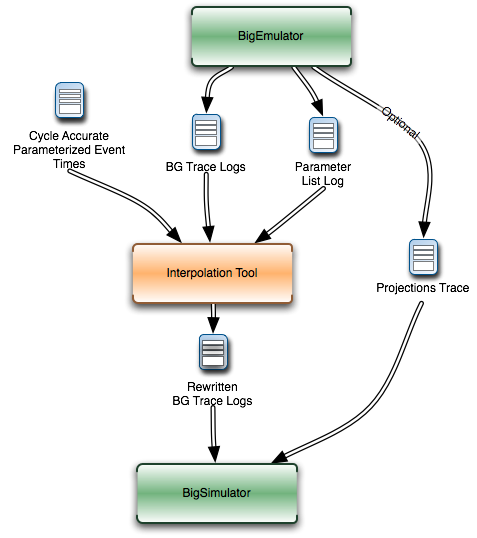
\includegraphics[width=4in]{figures/InterpolationFlow}
{\sffamily\bfseries\small \caption{Flow diagram for use of the interpolation tool\label{fig:interpolationflow}}}
\end{figure}

%%%%%%%%%%%%%%%%%%%%%%%%%%%%%%%%%%%%%%%%%%%%%%%%%%%%
\subsection{Tool Usage\label{usage}}

The interpolation tool is part of the regular \charmpp{} distribution and 
can be found under the directory \texttt{charm/examples/bigsim/tools/rewritelog} with a \texttt{README} file describing its use in more detail than this manual.

\subsubsection{Producing the Parameterized Timings Log}
The interpolation tool uses as input a log of actual durations of user-bracketed sequential execution blocks.
These timings come from a full or partial execution of the parallel application on a real machine or
within a cycle-accurate simulator. 

The user must insert \texttt{startTraceBigSim()} and  \texttt{endTraceBigSim()} calls around the main
computational regions in the parallel application. These two calls bracket the region of interest
and print out a record for that computational region. The functions should be called at most once during
any SEB. The output produced by  \texttt{endTraceBigSim()} is a line similar to

 ``\texttt{TRACEBIGSIM: event:\{ PairCalculator::bwMultiplyHelper \}  time:\{ 0.002586 \}  params:\{ 16384.00 1.00 220.00 128.00 128.00 0.00 0.00 0.00 \}}.'' 

\noindent
The event name and the values (in double-precision floating-point) for up to 20 parameters are
specified in the call to  \texttt{endTraceBigSim()}; the \texttt{time} field records  the duration of the bracketed region of sequential code. 

To run in a cycle-accurate simulator such as IBM's MAMBO, the  \texttt{startTraceBigSim()} and  \texttt{endTraceBigSim()} functions would be modified to switch between the ``fast forward'' mode used during the rest of the
program and the cycle-accurate mode during the bracketed region of code. The functions are provided in C++ source files under the directory \texttt{charm/examples/bigsim/tools/rewritelog/traceBigSim} and their calls
must be added to an application's source file manually.

%%%%%%%%%%%%%%%%%%%%%%%%%%%%%%%%%%%%%%%%%%%%%%%%%%%%
\subsubsection{The BigSim log file format}

To understand how the interpolation tool works, it is instructive to consider the format
of logs produced by the BigSim Emulator.
A BigSim log file (i.e. bgTrace log) contains data from emulation of the full parallel application.
There is an entry for each SEB, with the following fields:  \textit{ID}, \textit{Name}, $T_{start}$,
$T_{end}$, \textit{Back}, \textit{Forward}, \textit{Message ID}, \textit{Source Node},
\textit{Message ID}, \textit{Sent Messages}. The final field is actually a list of records for each
message sent by the execution block; each record contains the following fields:
 \textit{Message ID}, $T_{sent}$, $T_{recv}$, \textit{Destination PE}, \textit{Size}, \textit{Group}.

The interpolation tool will rewrite the durations of the SEBs by correcting the $T_{end}$ field for the
SEB and the $T_{sent}$ fields for each message sent. The new durations of all SEBs will be based upon
some model $M:SEB\rightarrow Duration$. 

Each SEB can be decomposed into three temporal regions as shown in Figure~\ref{event_diagram}. 
The entire SEB is associated with execution of a Charm++ entry method, while the middle region
is the computational kernel of interest, bracketed by the user's \texttt{startTraceBigSim()} and  \texttt{endTraceBigSim()} calls. The model is used only to approximate the new duration of the middle temporal region;
the durations of the beginning and ending regions are simply scaled by a constant factor.
Internally, the interpolation tool takes the ID for each SEB and looks up its associated parameters.
%If
When those parameters are found, they are used as input for evaluation of the new duration $d_{new}$
for the SEB. The end time is then modified to be $T_{end}\leftarrow  T_{start}+d_{new}$.

\begin{figure}
\centering
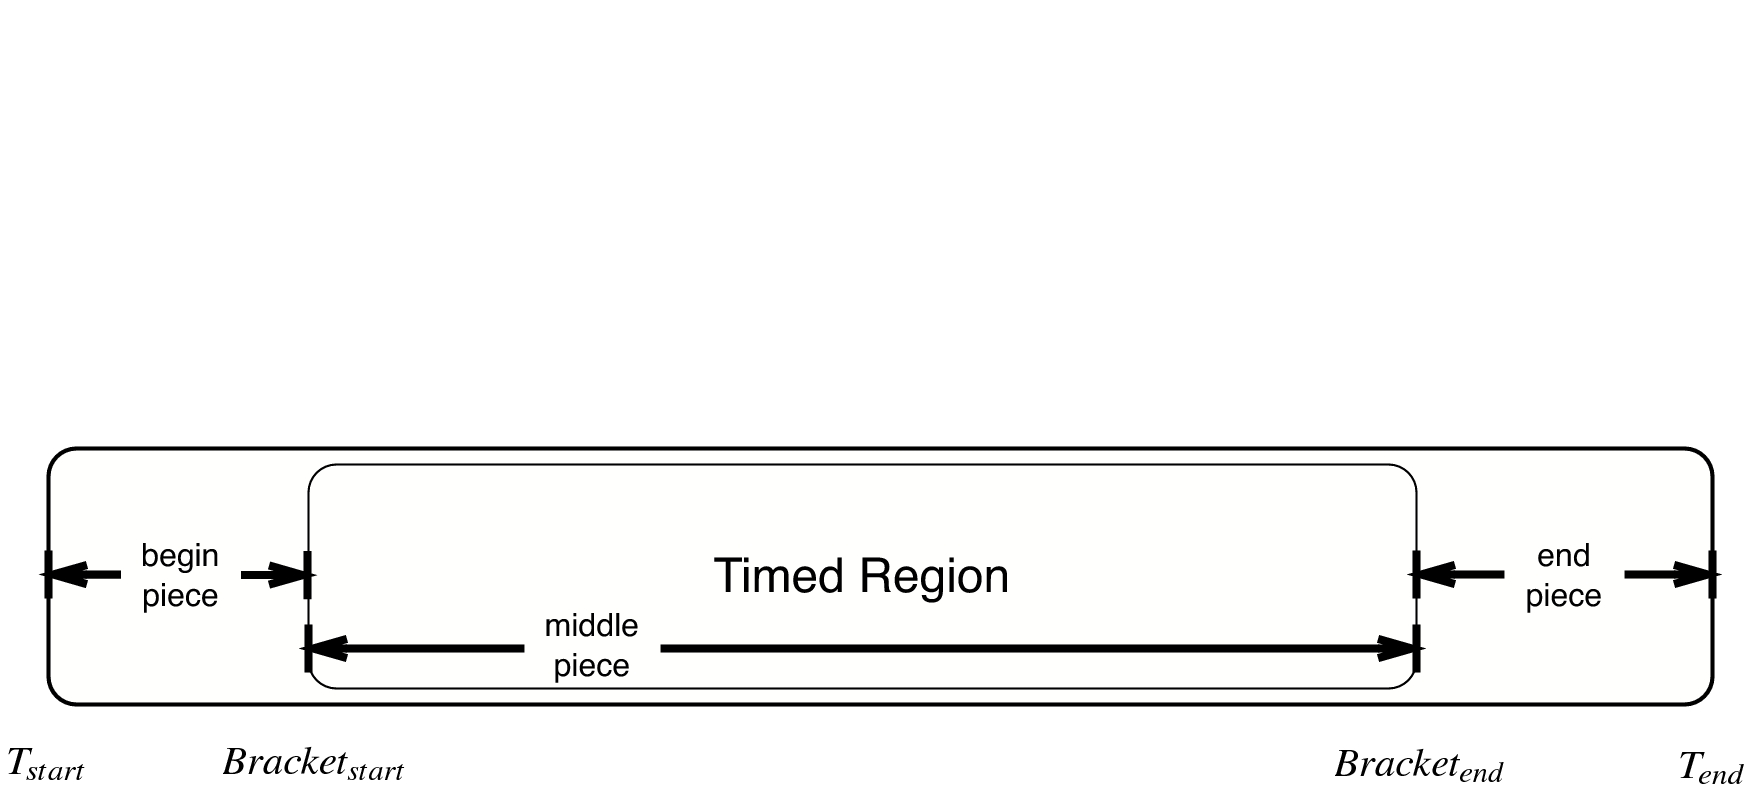
\includegraphics[width=5in]{figures/event_diagram}
\caption{SEBs in the bgTrace file have a start and end time. Only a portion of the SEB, e.g. the important compuational kernel, is timed when performing cycle accurate simulation. The duration of the middle portion of the SEB can be estimated in a different manner than the rest of the SEB. For example, the begin and end pieces can be scaled by some constant factor, while the bracketed middle region's duration can be estimated based on a more
sophisticated model.
\label{event_diagram}}
\end{figure}

\begin{figure}
\centering
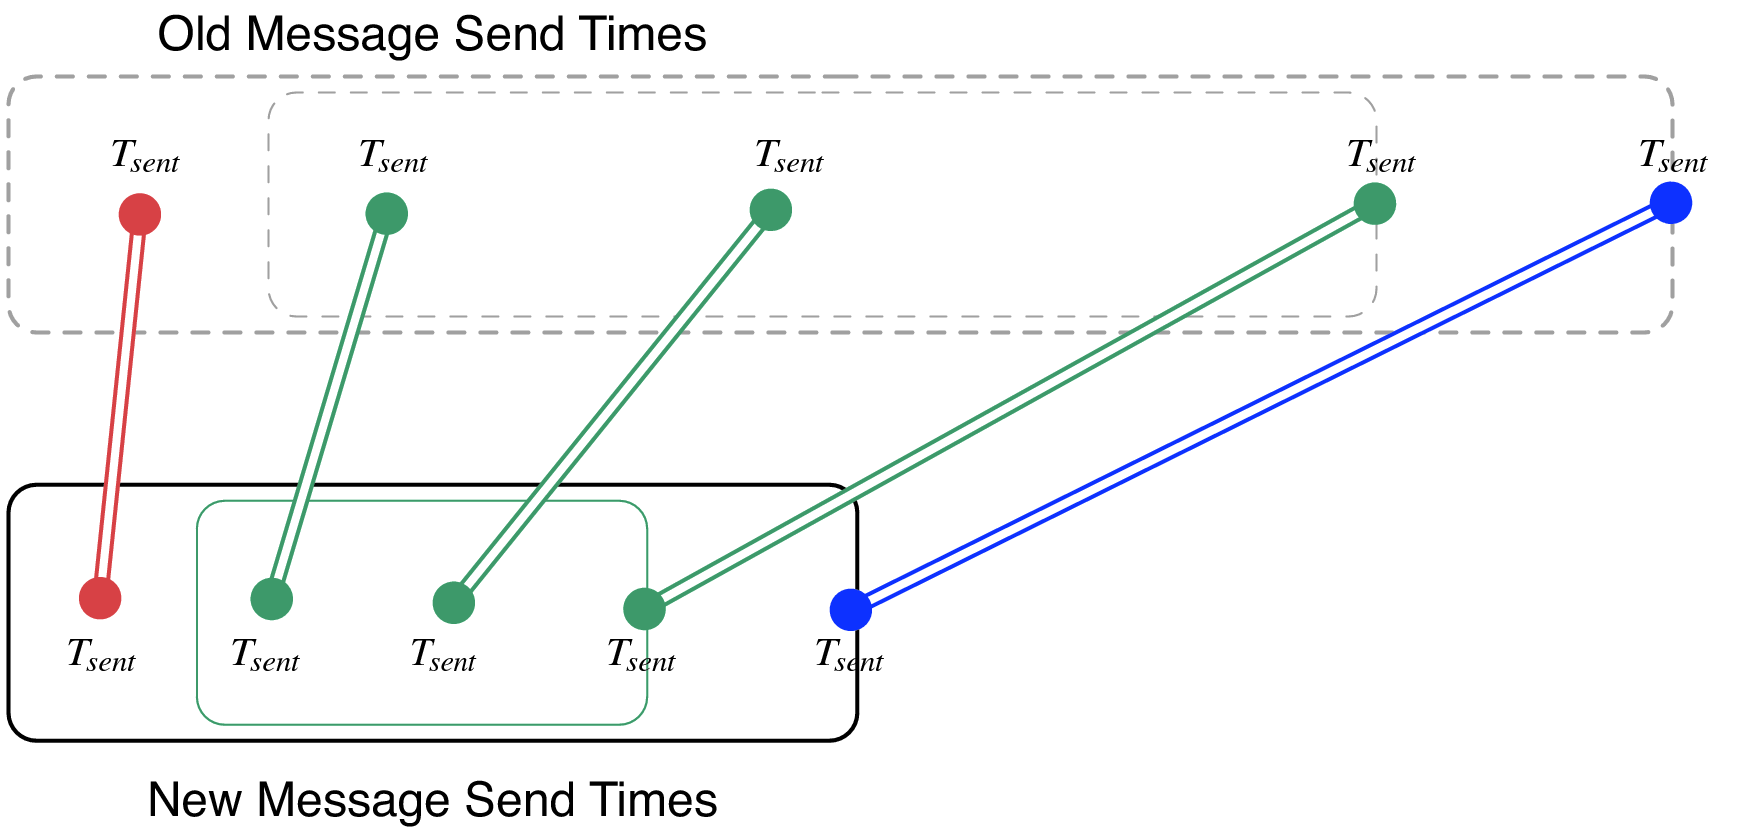
\includegraphics[width=6in]{figures/event_diagram2}
\caption{Message send times for messages sent from an SEB are remapped linearly onto the new time ranges for the 
SEB, region by region.
\label{event_diagram2}}
\end{figure}

The messages in the message list for each SEB must also have their $T_{sent}$ times rewritten. This is accomplished by linearly mapping the old $T_{sent}$ value from to the new range for the enclosing SEB region, as shown in Figure \ref{event_diagram2}. Any message sent during the first portion will be mapped linearly onto the new first portion of the SEB. The new message $T_{recv}$ times are ignored by BigSimulator, so they do not need to be modified.


\subsubsection{Supported performance models}
The interpolation tool supports three types of models, as described in this subsection.
% \ref{sec:model:scale}, \ref{sec:model:parameterization}, and \ref{sec:model:partial}. 
The more sophisticated models use the least-square curve fitting technique. 
The current implementation uses the Gnu Scientific Library(gsl) to perform the
least-square fit to the given data. The library provides both the coefficients and a $\chi^2$ measure of the closeness of the fit to the input data. 


%%%%%%%%%%%%%%%%%%%%%%%%%%%%%%%%%%%%%%%%%%%%%%%%%%%%
\paragraph{Model 1: Scaling SEB durations by a constant factor}
%\label{sec:model:scale}}

In simple cases, a sufficient approximation of the performance of a parallel application can be obtained
by simply scaling the SEB durations by a constant factor.
As an example, a user may know that a desired target machine has processors that will execute
each SEB twice as fast as on an existing machine.
The application is emulated on the existing machine and the observed SEB durations are scaled
by a factor of $2.0$. Although simple, this method may be sufficient in many cases. It becomes
unnecessary to use the \texttt{startTraceBigSim()} and  \texttt{endTraceBigSim()} calls.
The scaling factor is hard coded in the interpolation tool as \texttt{time\_dilation\_factor}.
It is used to scale all blocks unless a suitable advanced model has a better method for approximating the 
block's duration. It will always be used to scale any portions of blocks that are not bracketed with
the calls \texttt{startTraceBigSim()} and  \texttt{endTraceBigSim()}.

\paragraph{Model 2: Extrapolation based on user's parameterizations}
%\label{sec:model:parameterization}}

The user can simply insert the bracketing calls  \texttt{startTraceBigSim()} and
  \texttt{endTraceBigSim()} around the computational kernels to log the times taken for each kernel.
In practice, the duration of the SEB will likely depend upon the data distribution and access patterns
for the parallel application. Thus, the user must specify parameters likely to influence the SEB duration.
The parameters can include variables indicating number of loop iterations, number of calls to
computational kernels, or sizes of accessed portions of data arrays. A model is built to
approximate the duration of any SEB based upon its specified parameters.

As an example, NAMD uses a number of different types of objects. The \texttt{compute} objects will spend varying amounts of time depending upon the lengths of their associated atom lists. If an atom list is large, more interactions are computed and thus more computation is performed. 
% Now the method is described in the context of a simple hypothetical molecular dynamics application. 
Meanwhile, assume that a Charm++ entry method called \texttt{doWork(atomList)} is where the majority
of the work from an application occurs. The function computes forces on atoms of various types.
Different calls to the function will contain different numbers and types of atoms.
The source code for  \texttt{doWork(atomList)} will be modified by the user to  contain calls to
\texttt{startTraceBigSim()} at the entry and  \texttt{endTraceBigSim()} at the exit of the function.
The program will be run, and the resulting timed samples will be used to build a model. Assume the expected runtime of \texttt{doWork(atomList)} is quadratic in the \texttt{atomList} length and linear in the number of carbon atoms in the \texttt{atomList}. The \texttt{endTraceBigSim()}  call would be provided with a descriptive name and a set of parameters, such as \texttt{endTraceBigSim(``doWork()'', $p_1$,$p_2$)},  where parameter $p_1$ is the length of \texttt{atomList} and parameter $p_2$ is the number of carbon atoms in \texttt{atomList}.

The goal of using a model is to be able to predict the execution time of any arbitrary call to
\texttt{doWork()}, given its parameters. The application can be run on an existing processor
or parallel cluster for only a few timesteps with the modified \texttt{doWork()} method. 
This run will produce a list of \{$\left(p_1,p_2\right)\rightarrow duration$\} records. 
A least squares method is applied to fit a curve $f(p_1,p_2)=c_1+c_2 p_1+c_3 p_1^2 + c_4 p_2$  
approximating the durations of the records. The least square method minimizes the sum of the
squares of the difference between the function $f$ evaluated at each parameter set and the actual
timing observed at those parameters. The least square method is provided
 $\left(1.0,p_1,p_1^2,p_2,time\right)$ for each sample point and produces the coefficients $c_n$ in $f$. 
An arbitrary set of parameters (in the current implementation, up to twenty) can be input
to $f$ to produce an approximation of the runtime of \texttt{doWork()} even though the particular instance was never timed before. 

\paragraph{Model 3: Extrapolation of partial executions with cycle accurate simulations 
and user's parameterizations}
%\label{sec:model:partial}}

In this case, a cycle accurate simulator can be used to simulate a small fraction of all SEBs for a run
 of the application. The partial execution is used to build a model which applies to the whole execution.
Parameterizations can be used as 
% in section \ref{sec:model:parameterization}
previously described,
so that only some fraction of the SEBs will be run in the expensive cycle-accurate simulator. 
In NAMD, for example, a sufficient model can be built from  a random sample of 2\% of the cycle-accurate SEB durations from four timeloop iterations. 



\section{BigSim Log Generation API}
\label{bgapi}


To be added ...



\input{index}

\end{document}

